\chapter{Method} \label{CH4}
Run simulations of plates with defects using cheap FSI by multiplying the lagrangian pressure with cosine of angle. Train a ANN and see if it can replicate this cheap FSI, (it should pretty much 100\%). Integrate the neural net with abaqus.

Simulate the plate using fully coupled FSI in Europlexus. Train an AI on this. Evaluate. Investigate if the material properties can be accounted for in the neural net.

\
\begin{figure}
    \centering
    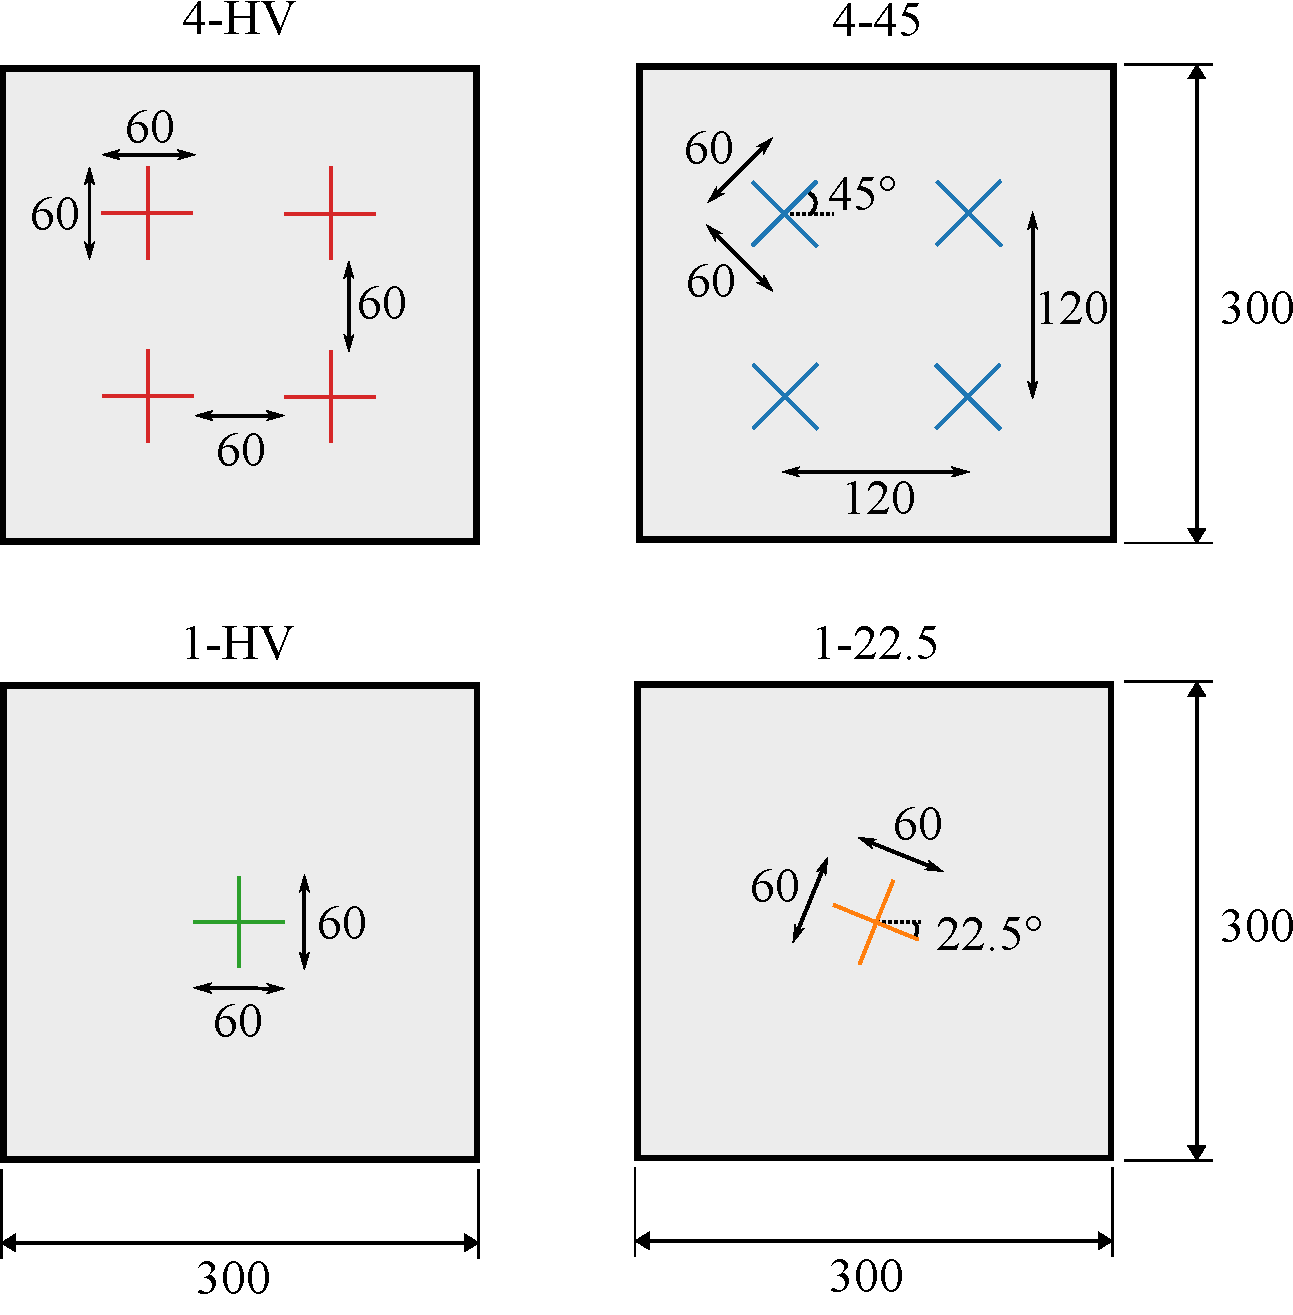
\includegraphics[width=.8\textwidth]{plates}
    \caption{Bottom text}
    \label{fig:plates}
\end{figure}

\begin{figure}
    \centering
    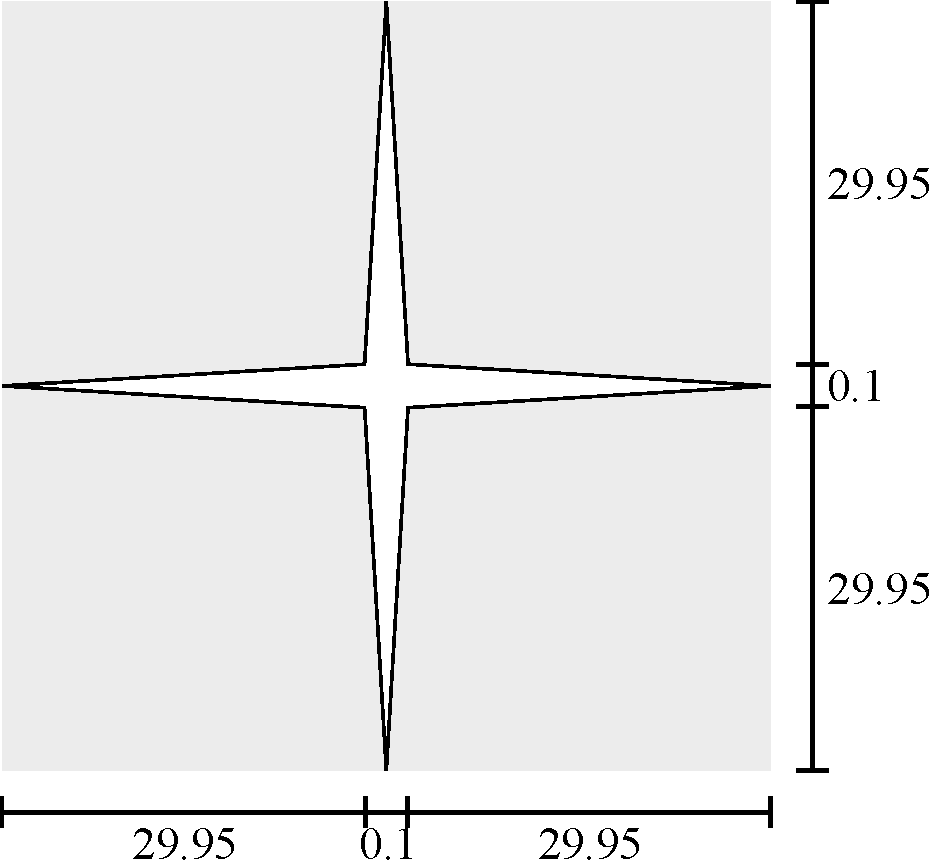
\includegraphics[width=.5\textwidth]{slit}
    \caption{Bottom text}
    \label{fig:slit}
\end{figure}

\begin{figure}
    \centering
    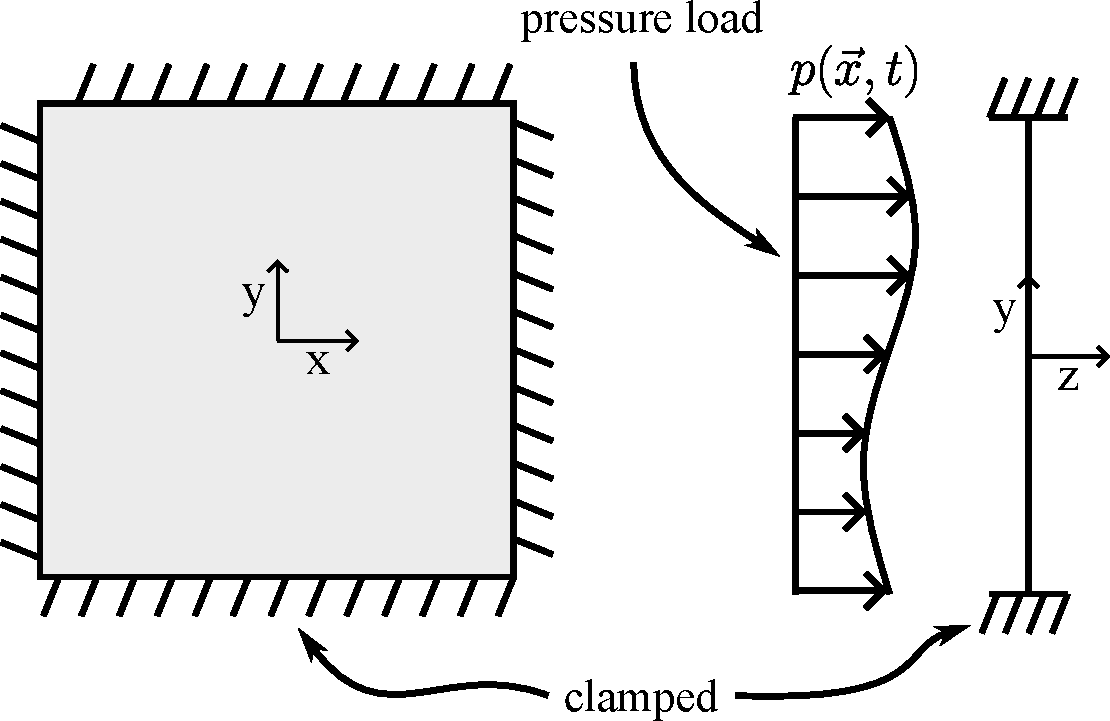
\includegraphics[width=\textwidth]{BC}
    \caption{Bottom text}
    \label{fig:bc}
\end{figure}